\documentclass[11pt]{article}
%%%%%%%%%%%% PREAMBULO %%%%%%%%%%%%%%%%%%
\usepackage[T1]{fontenc}%indica que usamos la ñ
\usepackage[utf8]{inputenc}%indica el tipo de codificación ISO-8859-1 (latin)ó utf8
\usepackage[spanish]{babel}%indica que escribiremos en español
\title{plantilla para reportes mecatrónica-mecánica UTA}
\usepackage{amsmath}
\usepackage{amssymb,amsfonts,latexsym}
\usepackage{graphicx}
\usepackage{epstopdf}%para convertir figuras a formato pdf
\usepackage{color}
\usepackage{url}  \urlstyle{same}%para conectar url strings en bibliografías
\usepackage{subfigure}%para colocar varias figuras
\usepackage{multicol}
\usepackage{changepage}
\usepackage{float}%para colocar las tablas como H
\usepackage{array}%dar formato a las tablas
\usepackage{longtable}%dar formato a las tablas
\usepackage{bm}
\usepackage{capt-of}
\usepackage{sidecap}
\sidecaptionvpos{figure}{c}
\usepackage{caption}
\usepackage{commath}
\usepackage{cancel}
\usepackage{lipsum}
%%%%%%%%%%% CONFIGURACION DEL DOCUMENTO %%%%%%%%%%%%%
\usepackage{anysize}%para personalizar el ancho de los margenes
\marginsize{2cm}{2cm}{2cm}{2cm}%izquierda, derecha, arriba, abajo
\usepackage{anyfontsize}

% Para que las referencias sean hipervínculos a las figuras o ecuaciones y
% aparezcan en color
\usepackage[colorlinks=true,plainpages=true,citecolor=blue,linkcolor=blue]{hyperref}
%\usepackage{hyperref} 
% Para agregar encabezado y pie de página
\usepackage{fancyhdr} 
\pagestyle{fancy}
\fancyhf{}
\fancyhead[L]{\footnotesize FICH} %encabezado izquierda
\fancyhead[R]{\footnotesize Centis Mateo}   % dereecha
\fancyfoot[R]{\footnotesize Entregable 1}  % Pie derecha
\fancyfoot[C]{\thepage}  % centro
\fancyfoot[L]{\footnotesize Ingeniería en informática}  %izquierda
\renewcommand{\footrulewidth}{0.4pt}
\usepackage{listings} % Para usar código fuente

% configuración para el lenguaje que queramos utilizar
\definecolor{mygreen}{rgb}{0,0.6,0}
\definecolor{mygray}{rgb}{0.5,0.5,0.5}
\definecolor{mymauve}{rgb}{0.58,0,0.82}
\definecolor{myorange}{rgb}{0.855,0.576,0.027}
\definecolor{backcolour}{rgb}{0.95,0.95,0.92}
\lstset{
language=Octave,
frame=single,   
morecomment = [l][\itshape\color{mygreen}]{\%},
keywordstyle=\color{blue},
commentstyle=\color{mygreen},	
breakatwhitespace=false,         
breaklines=true,  
%numbers=left,
%numbersep=5pt,
basicstyle=\linespread{0.9}\ttfamily\small,
%numberstyle=\tiny\color{mygray}, 
showstringspaces=false, 
showtabs=false,                  
tabsize=2,
stringstyle=\color{myorange},
title=\lstname,
literate=
{+}{{{\color{red}+}}}1
{-}{{{\color{red}-}}}1
{*}{{{\color{red}*}}}1
{,}{{{\color{red},}}}1
{=}{{{\color{red}=}}}1
{)}{{{\color{red})}}}1
{(}{{{\color{red}(}}}1 
{;}{{{\color{red};}}}1
{:}{{{\color{red}:}}}1
{[}{{{\color{red}[}}}1
{]}{{{\color{red}]}}}1
{>}{{{\color{red}>}}}1
}
\title{Plantilla para informes ing. mecanica-mecatronica}

%%%%%%%%%%% COMIENZO DEL DOCUMENTO %%%%%%%%%%%%
\begin{document}

%%%%%%%%%%%%%%%%%%%%%%%%%%%%%%%%%% PORTADA %%%%%%%%%%%%%%%%%%%%%%%%%%%%%%%%%%%%%%%%%%%%

\begin{center}																		%%%
  \newcommand{\HRule}{\rule{\linewidth}{0.5mm}}									%%%\left

  %%%

  %%%
  \vspace*{1.0cm}								%%%
  %%%	
  \textsc{\huge UNL - FICH \vspace{5px}}\\[1.5cm]

  \textsc{\LARGE Cálculo numérico - Entregable 2}\\[1.5cm]													%%%

  \textsc{\LARGE Centis Mateo}

\end{center}

%%%%%%%%%%% CUERPO DEL DOCUMENTO
\section*{Enunciado}
La energía térmica total de un dispositivo está dada por la expresión
$E(t)=((t+\frac{1}{3})^3+\frac{1}{3})e^{-t}$ para cada instante de tiempo t.
\begin{enumerate}
  \renewcommand{\theenumi}{\alph{enumi}} %Letras minúsculas
  \item Determinar los instantes de tiempo en los que la energía del dispositivo
        es igual a 1.5, con 5 dígitos de precisión.
  \item Determinar la máxima energía del sistema y en qué tiempo ocurre, utilizando
        la misma precisión que en item anterior.
  \item Determinar el instante de tiempo en dónde se da la máxima tasa de crecimiento
        instantánea de la energía respetando la precisión anterior.
\end{enumerate}
Justificar cuál método eligió para resolver cada inciso, destacando las ventajas del mismo.
\newpage
\section*{Resolución}
\subsection*{(a)}
Se debe realizar la búsqueda de los instantes de tiempo dónde E(t) sea igual a 1.5, es decir,
$E(t)=1.5$. Para esto se creó una nueva función $f(t)=E(t)-1.5$. Y se la igualó a cero para poder
utilizar los métodos vistos en la materia. Al realizar la gráfica de la función es posible observar
que existen dos raíces entre los intervalos [1,2] y [3.5,4.5].
\begin{figure}[!h]
  \centering
  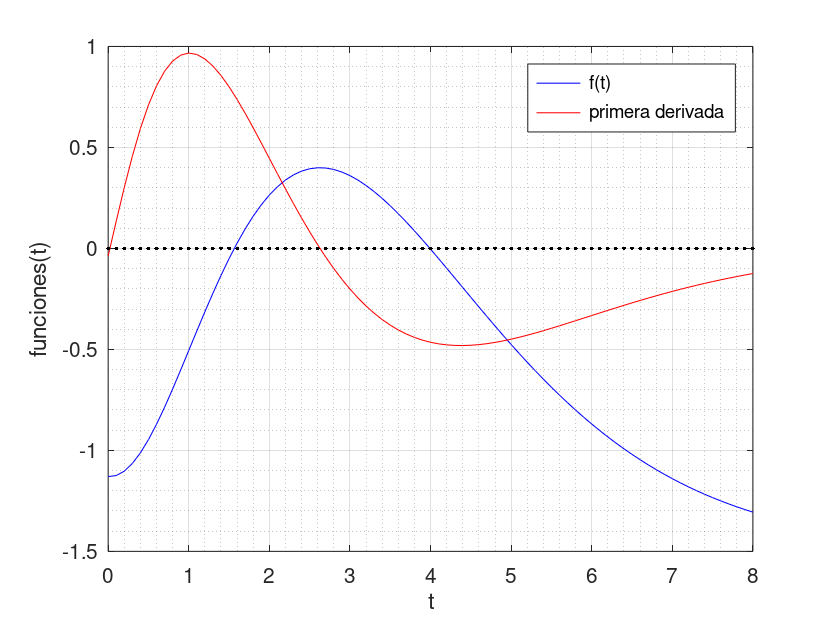
\includegraphics[scale=0.5]{incisoA.png}
\end{figure}

Para decidir que método utilizar se realizó la derivada de la función $f(t)$, y se encontró
$f'(t)=-e^{-t}((t+\frac{1}{3})^3+\frac{1}{3})+3e^{-t}(t+\frac{1}{3})^2$.
Se decidió usar el método de Newton-Raphson para encontrar las raíces, esto se debe a
que tenemos una buena aproximación inicial y podemos asegurar su convergencia,
ya que su derivada es distinta de cero entre los intervalos buscado y además,  $f(p)=0$ y $f'(p)\ne 0$ en ambos p buscados,
por lo que son raíces simples y por ende el orden de convergencia del método va a ser cuadrático.
Utilizando la tolerancia en valor relativo para detener las iteraciones, se llegó
a las raíces $xNew_{11}=1.5649$ y $xNew_{12}=3.9924$ en 4 iteraciones.

\newpage
\subsection*{(b)}
Para determinar la máxima energía del sistema, se buscó el punto dónde la derivada de la función
se anule, es decir, su raíz. Se graficó la función para localizar el intervalo dónde se encuentra el punto
buscado y se puede notar como este se encuentra en el intervalo [2,3].
\begin{figure}[!h]
  \centering
  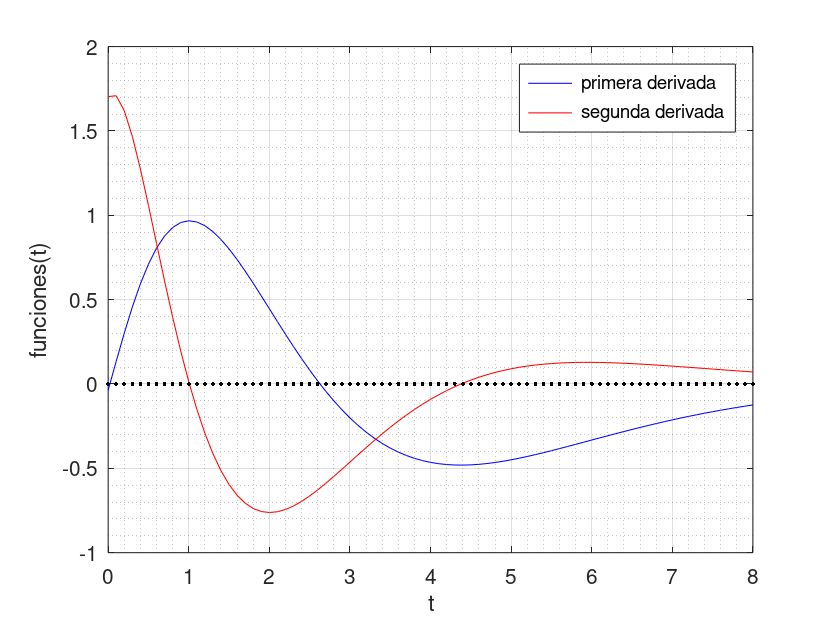
\includegraphics[scale=0.5]{incisoB.png}
\end{figure}

Se derivó nuevamente la función para obtener $f''(t)=\frac{e^{-t}(27t^3-135t^2+63t+46)}{27}$
y utilizando un razonamiento similar al usado en el inciso anterior se puede observar que cumple con las condiciones
para aplicar el método de Newton-Raphson. Aplicando el método con aproximación inicial $x_{02}=2.5$ y utilizando mismos
criterios para detener las iteraciones se obtuvo la solución $xNew_{2}=2.6287$ en 3 iteraciones.
\newpage
\subsection*{(c)}
Se desea determinar el instante de tiempo en dónde se de la máxima tasa de crecimiento instantánea
de la energía, es decir, encontrar el valor dónde la derivada de la función es máxima. Esto es equivalente
a buscar las raíces de la segunda derivada de la función, ya que los máximos de $f'(t)$ son los puntos dónde
cambia la concavidad de la $f(t)$ original, es decir, los puntos $p$ tales que $f''(p)=0$.

Se procedió de forma análoga al inciso anterior y se empezó por graficar $f''(t)$.
Al examinarla se puede ver a simple vista que existe una raíz en el intervalo [4,5].

\begin{figure}[!h]
  \centering
  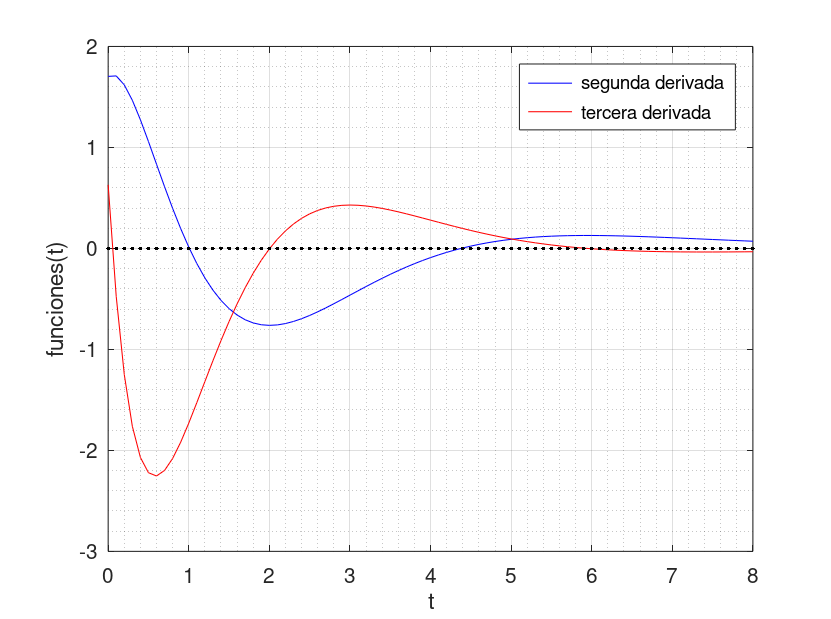
\includegraphics[scale=0.5]{incisoC.png}
\end{figure}
%En este parrafo se podría mencionar porque funciona newton
Para encontrar la raíz se utilizó una combinación de los métodos de la bisección y de
Newton-Raphson. En primer lugar, se buscó la raíz por bisección en el intervalo [1,2]
con una tolerancia mayor $tol_{bis}=1e-3$, para luego utilizar Newton-Raphson desde el punto retornado
por bisección, con una tolerancia menor. Procediendo de esta manera, se encontró por bisección el punto
$xBis=1.0083$ luego de 11 iteraciones y utilizándolo en Newton-Raphson se encontró como resultado
$xNew_3=1.0079$ luego de 2 iteraciones, teniendo como máxima tasa de decrecimiento $f'(xNew_3)=0.9674.

\newpage
\begin{center}																		%%%
  \newcommand{\HRule}{\rule{\linewidth}{0.5mm}}									%%%\left
  \vspace*{1.0cm}								%%%
  %%%	
  \textsc{\huge \underline{ANEXO} \vspace{5px}}\\
\end{center}

\begin{lstlisting}[caption={newton.m}]
function [x h1 i] = newton(f,df,x0,kmax,tol)
  i=1;
  while i < kmax
    x=x0-f(x0)/df(x0);
    h1 = abs(x-x0);%Cambiar a necesidad de error
    h2 = abs(x-x0)/abs(x);
    h3 = abs(f(x));
    if h1 < tol 
      return;
    endif
    i++;
    x0=x;
  endwhile
  disp('No converge en maximas iteraciones')
endfunction
\end{lstlisting}

\begin{lstlisting}[caption={biseccion.m}]
function [p h2 i] = biseccion(f,a,b,kmax,tol)
  %a y b son [a,b] 
  %h es la convegencia<
  i=1;
  while i < kmax
    p = a + (b-a)/2;
    h1=f(p);%Elegir que convergencia usar
    h2=abs(b-a);
    h3=abs(b-a)/2;
    if h2<=tol 
      return
    endif
    i++;
    if f(b)*f(p) < 0
      a = p;
    else 
      b = p;
    endif
  endwhile
  display('Iteraciones maximas alcanzadas')
endfunction
\end{lstlisting}

\begin{lstlisting}[caption={G4Ej7.m}]
  E=@(t)((t+1/3).^(3)+1/3).*e.^(-t);%Ecuacion de energia
  tol=1e-5;
  kmax=1000;
  %funciones y sus derivadas
  f=@(t)((t+1/3).^(3)+1/3).*e.^(-t)-1.5;%funcion de (a)
  df=@(t) -e.^(-t).*((t+1/3).^(3)+1/3)+3*e.^(-t).*(t+1/3).^(2);
  ddf=@(t)(e.^(-t).*(27*t.^3-135.*t.^2+63.*t+46))/27;
  dddf=@(t)(1/27).*(-333.*t.*e.^(-t)+
  216.*t.^2.*e.^(-t)-27.*t.^3.*e.^(-t)+17.*e.^(-t));
  t=[0:0.1:8];
  Et = E(t);
  dft = df(t);
  ddft=ddf(t);
  dddft = dddf(t);
  %----------------------------------------------------------------------
  %(a) Determinar instantes de tiempo en los que la energia es 
  %igual a 1.5, con 5 digitos de precision
  %Grafica de f(t)
  ft=f(t);
  figure(1)
  plot(t,ft,'b');
  hold on
  plot(t,dft,'r');
  hold on
  plot(t,0,'k')
  set(gca,'XTick',0:1:100)
  grid on
  grid minor
  xlabel('t')
  ylabel('funciones(t)')
  legend('f(t)','primera derivada')
  hold off
  %solucion por Newton-Raphson
  %intervalo 1
  x011=1;
  [xNew11 hNew11 itNew11] = newton(f,df,x011,kmax,tol)
  %intervalo 2
  x012=3.5;
  [xNew12 hNew12 itNew12] = newton(f,df,x012,kmax,tol)
  %----------------------------------------------------------------------
  %(b)Determinar max energia del sistema y en que t ocurre, utilizando
  %misma tol
  %Grafica de df(t)
  figure(2)
  plot(t,dft,'b');
  hold on
  plot(t,ddft,'r');
  hold on
  plot(t,0,'k');
  set(gca,'XTick',0:1:100)
  grid on
  grid minor
  xlabel('t')
  ylabel('funciones(t)')
  legend('primera derivada','segunda derivada')
  hold off
  %solucion por Newton-Raphson
  x02=2.5;
  [xNew2 hNew2 itNew2] = newton(df,ddf,x02,kmax,tol)
  %----------------------------------------------------------------------
  %(c) Determinar t en donde se da la max tasa de 
  %crecimiento instantanea de la energia con misma tol
  %Grafica de ddf(t)
  figure(3)
  plot(t,ddft,'b');
  hold on
  plot(t,dddft,'r');
  hold on
  plot(t,0,'k');
  set(gca,'XTick',0:1:100)
  grid on
  grid minor
  xlabel('t')
  ylabel("funciones(t)")
  legend('segunda derivada','tercera derivada')
  hold off
  %busqueda por biseccion
  tolBis = 1e-3;
  [xBis hBis itBis] = biseccion(ddf,1,2,kmax,tolBis)
  %solucion por newton-raphson
  [xNew3 hNew3 itNew3] = newton(ddf,dddf,xBis,kmax,tol)  
\end{lstlisting}

\end{document}

